%\documentclass[notes,usenames,dvipsnames]{beamer}
%\documentclass[notes]{beamer}       % print frame + notes
%\documentclass[notes=only]{beamer}   % only notes
\documentclass[usenames,dvipsnames]{beamer}             % only frames
\usepackage[outputdir=out]{minted}
\usepackage{pgfpages}
%\setbeameroption{show notes on second screen}
%\setbeameroption{show notes}
%subfigures
\usepackage{caption}
\usepackage{subcaption}

%tables packages
\usepackage{multirow}

% math
\usepackage{amsmath}

% bash command
\usepackage{graphicx}
\usepackage{listings}
% varbatim for ascii figures
\usepackage[T1]{fontenc}
\usepackage[utf8]{inputenc}
%\usepackage{verbatim}
\usepackage{lipsum} % for context
\usepackage{fancyvrb}
\usepackage{varwidth}
\usepackage{circuitikz}
\ctikzset{logic ports=ieee}
\usepackage{listings}
% \lstset{language=[Motorola68k]Assembler,basicstyle=\ttfamily,keywordstyle=\color{blue}}

\usepackage{shellesc}
\usepackage{adjustbox}

\newsavebox{\asciigcn}

% notes prefixed in pympress
\addtobeamertemplate{note page}{}{\thispdfpagelabel{notes:\insertframenumber}}
%theme used
\usetheme{Madrid}
%Information to be included in the title page:
\title[Computer Architecture] %optional
{Computer Architecture}

\subtitle{Course no. 8 - Interupts Systems}

\author[Ștefan-Dan Ciocîrlan] % (optional, for multiple authors)
{}

\institute[NUSTPB] % (optional)
{
  \inst{}%
  National University of Science and Technology\\
  POLITEHNICA Bucharest
}

\date[NUSTPB 2024] % (optional)
{Computer Architecture}

\logo{

\includegraphics[height=0.9cm]{../../media/LOGO_UNSTPB_en.png}

\includegraphics[height=0.9cm]{../../media/logoACSQ.jpeg}
}


% Roman numerals
\newcommand*{\rom}[1]{\expandafter\@slowromancap\romannumeral #1@}
%split
\usepackage{amsmath}
%colors
%\usepackage[usenames,dvipsnames]{color} %loaded by the dcoument class
%subfigure
\usepackage{subcaption}
% block over block uncover
\setbeamercovered{invisible}
%\setbeamercovered{transparent}

%extra slide content
\AtBeginSection[]
{
  \begin{frame}
    \frametitle{Content}
    \tableofcontents[currentsection]
  \end{frame}
}
%notes or not
%\setbeamertemplate{note page}[plain]

\begin{document}

\frame{\titlepage}

\section{Interupts Systems}

\begin{frame}
    \frametitle{Pooling Problems}
    \begin{itemize}
        \item It consumes a lot of CPU time
        \item It is not efficient, because it depends on the pooling time
        \begin{itemize}
            \item If the pooling time is too short, the CPU will consume a lot of time
            \item If the pooling time is too long, it delays the response time to the I/O devices
        \end{itemize}

        \item It is synchronous and it is not a good solution for real-time systems (It is a need for an asynchronous solution)

    \end{itemize}
\end{frame}

\begin{frame}
    \frametitle{Interrupts Systems}
    \begin{itemize}
        \item Asyncrhonous system
        \item Control and syncronize the asynchronous events in the system
        \item \textbf{Definition:} An interrupt is a signal to the processor emitted by hardware or software indicating an event that needs immediate attention
        \item \textbf{How it Works:} When a device needs service, it sends an interrupt signal. The CPU suspends its current task, processes the interrupt via an Interrupt Service Routine (ISR), and then resumes its previous work.
        \item \textbf{Advantages:}
        \begin{itemize}
            \item \textbf{Efficiency:} The CPU only handles the device when it is needed, freeing it up for other tasks.
            \item \textbf{Responsive System:} The system can quickly respond to time-sensitive events.

            \item \textbf{Better Multitasking:} Interrupts enable systems to handle \\ multiple tasks effectively without wasting CPU cycles.

        \end{itemize}
    \end{itemize}
\end{frame}

\begin{frame}
    \frametitle{Types of Interrupts}
        \begin{itemize}
            \item \textbf{Hardware Interrupts:} Generated by hardware devices or CPU.
            \item \textbf{Software Interrupts:} Generated by a program.
            \item \textbf{Maskable Interrupts:} Can be disabled or enabled.
            \item \textbf{Non-Maskable Interrupts:} Cannot be disabled.
            \item \textbf{Internal Interrupts:} Generated by the CPU itself.
            \item \textbf{External Interrupts:} Generated by external devices.
        \end{itemize}
\end{frame}

\begin{frame}
    \frametitle{Interrupts Systems Concepts}
    \begin{itemize}
        \item Classes of Interrupts, depending on source of the interupt we have different levels of interrupts
        \item Order of Priority, the CPU must know which interrupt to handle first
        \item Identification of the Interrupt, the CPU must known the level of the interrupt and if present order of priority in that level.
        \item Critical section of code where interupts are disabled. The interupts can be globally or specifically disabled.
        \item A save and restore context of the CPU, the CPU must save the context of the current task and restore it after the interrupt is handled.
        \item Comunication between the CPU and the I/O devices.
        \item Time of the interrupt. It must be as short as possible.
    \end{itemize}
\end{frame}

% Slide 1: Overview of Interrupt Handling Mechanism
\begin{frame}
    \frametitle{Interrupt Handling Mechanism: Overview}
    \begin{itemize}
        \item Interrupt Request (IRQ) Lines
        \item Interrupt Vector Table (IVT)
        \item Interrupt Service Routines (ISRs)
        \item Prioritization and Nesting
        \item Context Switching
    \end{itemize}
\end{frame}

% Slide 2: Interrupt Request (IRQ) Lines
\begin{frame}
    \frametitle{Interrupt Request (IRQ) Lines}

    \begin{itemize}
        \item \textbf{Definition}: IRQ lines are dedicated hardware lines used by I/O devices to signal the CPU.
        \item \textbf{Functionality}: When a device needs attention, it sends an IRQ signal, alerting the CPU.
        \item \textbf{CPU Response}: The CPU identifies the source of the interrupt and initiates the appropriate Interrupt Service Routine (ISR).
    \end{itemize}
\end{frame}

% Slide 3: Interrupt Vector Table (IVT)
\begin{frame}
    \frametitle{Interrupt Vector Table (IVT)}

    \begin{itemize}
        \item \textbf{Definition}: The IVT is a table in memory that holds jumps instruction to addresses of Interrupt Service Routines (ISRs).
        \item \textbf{Purpose}: Provides a quick way to look up and execute the correct ISR based on the interrupt.
        \item \textbf{Mechanism}: When an interrupt occurs, the CPU retrieves the ISR address from the IVT and jumps to that address to execute the instruction which starts the ISR.
    \end{itemize}
\end{frame}

% Slide 4: Interrupt Service Routine (ISR)
\begin{frame}
    \frametitle{Interrupt Service Routine (ISR)}

    \begin{itemize}
        \item \textbf{Definition}: An ISR is a special function that executes in response to an interrupt.
        \item \textbf{Purpose}: Handles the specific task associated with the interrupt (e.g., data transfer, status update).
        \item \textbf{Execution Flow}:
            \begin{itemize}
                \item usually disable interrupts at the beginning of the ISR. (cli)
                \item Execute the ISR code.
                \item last instruction of the ISR is a return from interrupt instruction. (reti) (enable interrupts)
            \end{itemize}
    \end{itemize}
\end{frame}

% Slide 5: Prioritization and Nesting
\begin{frame}
    \frametitle{Prioritization and Nesting}

    \begin{itemize}
        \item \textbf{Prioritization}: High-priority interrupts can preempt lower-priority ones, allowing critical events to be addressed immediately.
        \item \textbf{Nesting}: Allows multiple interrupts to be handled simultaneously, where an interrupt may trigger another.
        \item \textbf{Benefits}: Enhances system responsiveness and ensures critical events are handled first.
    \end{itemize}
\end{frame}

% Slide 6: Context Switching
\begin{frame}
    \frametitle{Context Switching in Interrupt Handling}

    \begin{itemize}
        \item \textbf{Definition}: Saving the CPU's current state (registers, program counter) before handling an interrupt.
        \item \textbf{Process}:
            \begin{enumerate}
                \item Save the context of the interrupted task.
                \item Execute the ISR.
                \item Restore the context after ISR completion.
            \end{enumerate}
        \item \textbf{Importance}: Ensures that the CPU resumes its previous task exactly where it left off.
    \end{itemize}
\end{frame}

\section{Implementation}
\begin{frame}
    \frametitle{Implementation for Lab CPU}
    \textbf{Type of interrupts:}
    \begin{itemize}
        \item Internal interrupts (non-maskable):
        \begin{itemize}
            \item ALU overflow
            \item Software interrupt through the \texttt{INT} instruction
        \end{itemize}
        \item External non-maskable interrupts:
        \begin{itemize}
            \item Lack of Voltage (Power Off)
            \item Special hardware line \texttt{cinm}
        \end{itemize}
        \item External maskable interrupts:
        \begin{itemize}
            \item 8 IO deivce interrupts
            \item Special hardware line \texttt{cintr} for all.
        \end{itemize}
    \end{itemize}
\end{frame}

\begin{frame}
    \frametitle{Implementation of IVT}
    \begin{table}[]
        \resizebox{0.9\textwidth}{!}{%
            \begin{tabular}{|c|c|c|}
                \hline
                \textbf{Address} & \textbf{Name} & \textbf{Type} \\ \hline
                0x0 & Reserved  & \multirow{3}{*}{Internal Interrupt} \\ \cline{1-2}
                0x1 & Software Interrupt (INT) & \\ \cline{1-2}
                0x2 & ALU Overflow & \\ \hline
                0x3 & Lack of Voltage (Power Off) & External Non-Maskable Interrupt \\ \hline
                0x4 & Level 0 & \multirow{8}{*}{External Maskable Interrupt} \\ \cline{1-2}
                0x5 & Level 1 & \\ \cline{1-2}
                0x6 & Level 2 & \\ \cline{1-2}
                0x7 & Level 3 & \\ \cline{1-2}
                0x8 & Level 4 & \\ \cline{1-2}
                0x9 & Level 5 & \\ \cline{1-2}
                0xA & Level 6 & \\ \cline{1-2}
                0xB & Level 7 & \\ \hline
            \end{tabular}
        }
    \end{table}
    \note{
    }

\end{frame}

\begin{frame}
    \frametitle{Interupt Instructions}
    The FR (Flag Register) will have a new bit \texttt{I} which will be used to enable or disable interrupts.
    The following instructions will be added:
    \begin{itemize}
        \item \texttt{EI} - Enable interrupts (sei)
        \item \texttt{DI} - Disable interrupts (cli)
        \item \texttt{INT} - Genrate software interrupt
        \item \texttt{RETI} - Return from interrupt
    \end{itemize}
\end{frame}

\begin{frame}
    \frametitle{Architecture}
    \begin{figure}
        \centering
        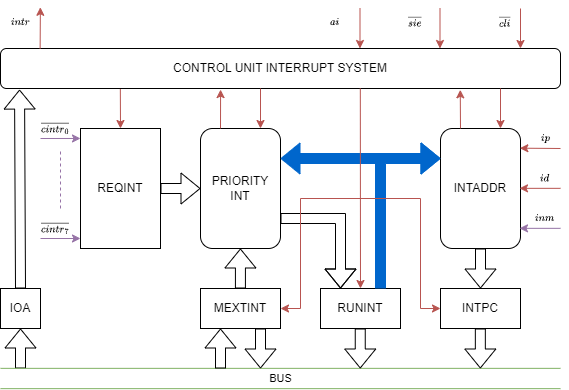
\includegraphics[width=0.8\textwidth]{media/isarchitecture.png}
    \end{figure}
\end{frame}

\begin{frame}
    \frametitle{Architecture Signals}
    \begin{itemize}
        \item $ip$ - Software Interrupt
        \item $id$ - ALU Overflow Interrupt
        \item $inm$ - external non-maskable interrupt (comes from $cinm$)
        \item $cintr_{i}$ - external maskable interrupt from device $i$
        \item $ai$ - external maskable interrupt active
        \item $intr$ - external maskable interrupt request to CPU
        \item $sie$/$cie$ - enable/disable external maskable interrupts
    \end{itemize}
\end{frame}

\begin{frame}
    \frametitle{Architecture Components}
    \begin{itemize}
        \item \texttt{REQINT} - Request external maskable interrupt register ($REQINT_{i} = 1$ means that the interrupt $i$ is requested)
        \item \texttt{MEXTINT} - Maskable external interrupt register ($MEXTINT_{i} = 1$ means that the interrupt $i$ is masked)
        \item \texttt{RUNINT} - Current running interrupts register ($RUNINT_{i} = 1$ means that the interrupt on level $i$ is running)
        \item \texttt{Priorrity INT} - Compute if the current interrupt has higher priority than the current running interrupt
        \item \texttt{INTADDR} - Compute the address of the ISR
        \item \texttt{INTPC} - The address for the current ISR
    \end{itemize}
\end{frame}

\begin{frame}
    \frametitle{External maskable interrupts Handling}
    \begin{enumerate}
        \item Verify for external maskable interrupt requests in the \texttt{REQINT} register.
        \item If there is one, verify if external maskable interrupts are enabled. (flag \texttt{I} in FR)
        \item If yes, filter the interrupts that are masked in the \texttt{MEXTINT} register.
        \item Find the highest priority interrupt that is not masked.
        \item Verify if it has higher priority than the current running interrupts in the \texttt{RUNINT} register:
        \item Send the interrupt to the CPU through the $intr$ signal.
        \item Wait for the CPU to acknowledge the interrupt. ($ai$ signal)
        \item Set the bit in the \texttt{RUNINT} register.
        \item Clear the bit in the \texttt{REQINT} register.
        \item Compute the address of the ISR and set the \texttt{INTPC} register.
    \end{enumerate}
\end{frame}

\begin{frame}
    \frametitle{External non-maskable interrupts Handling}
    \begin{enumerate}
        \item Verify for external non-maskable interrupt requests in the \texttt{inm} signal.
        \item Verify if there is no higher priority interrupt running.
        \item Compute the address of the ISR and set the \texttt{INTPC} register.
    \end{enumerate}
\end{frame}

\begin{frame}
    \frametitle{ALU Overflow Handling}
    \begin{enumerate}
        \item Verify for ALU overflow interrupt requests in the \texttt{id} signal.
        \item Verify if there is no higher priority interrupt running.
        \item Compute the address of the ISR and set the \texttt{INTPC} register.
        \item Inside the ISR, the CPU must clear the  overflow flag in the FR.
    \end{enumerate}
\end{frame}

\begin{frame}
    \frametitle{Software interrupts Handling}
    \begin{enumerate}
        \item Verify for software interrupt requests in the \texttt{ip} signal.
        \item There is no higher priority interrupt running.
        \item Compute the address of the ISR and set the \texttt{INTPC} register.
    \end{enumerate}
\end{frame}

\begin{frame}
    \frametitle{CPU acknowledge interrupts}
    \begin{enumerate}
        \item Save FR on the stack.
        \item Disable external maskable interrupts. (\texttt{EI} can be used to enable them back inside ISR)
        \item Save the current PC on the stack.
        \item Run the jump instruction from the \texttt{INTPC} register address.
    \end{enumerate}
\end{frame}

\begin{frame}
    \frametitle{Exam Questions}
    Template: Having the following values in the registers at time 0,
    interrupts requested with the time of the request and the type of the interrupt,
    and how much time the CPU will take to handle every type of interrupt,
    which is the order of the interrupts that will be handled by the CPU?
\end{frame}


\begin{frame}
    \frametitle{Exam Questions}
    \begin{table}[]
        \begin{tabular}{|c|c|c|c|}
            \hline
            \texttt{REQINT} & \texttt{MEXTINT} & \texttt{RUNINT} & \texttt{FR} \\ \hline
            0x00 & 0x00 & 0x00 & 0x00 \\ \hline
        \end{tabular}
    \end{table}

    \begin{table}[]
        \begin{tabular}{|c|c|c|c|}
            \hline
            Cycles from time 0 & Type of Request & Name \\ \hline
            10 & External Maskable Interupt Level 5 & A \\ \hline
            30 & External Maskable Interupt Level 3 & B \\ \hline
            50 & External Maskable Interupt Level 7 & C \\ \hline
            60 & External Maskable Interupt Level 1 & D \\ \hline
            100 & External Non-Maskable Interupt & E \\ \hline
            140 & ALU Overflow & F \\ \hline
            150 & Software Interupt & G \\ \hline
        \end{tabular}
    \end{table}
\end{frame}



\begin{frame}
    \frametitle{Exam Questions}
    \begin{table}
        \begin{tabular}{|c|c|c|c|}
            \hline
            Type of Request & Cycle to handle \\ \hline
            External Maskable Interupt Level 0 & 30 \\ \hline
            External Maskable Interupt Level 1 & 20 \\ \hline
            External Maskable Interupt Level 2 & 10 \\ \hline
            External Maskable Interupt Level 3 & 40 \\ \hline
            External Maskable Interupt Level 4 & 20 \\ \hline
            External Maskable Interupt Level 5 & 30 \\ \hline
            External Maskable Interupt Level 6 & 10 \\ \hline
            External Maskable Interupt Level 7 & 20 \\ \hline
            External Non-Maskable Interupt & 5 \\ \hline
            ALU Overflow & 10 \\ \hline
            Software Interupt & 10 \\ \hline
        \end{tabular}
    \end{table}
\end{frame}



\begin{frame}
    \frametitle{Exam Questions}
\end{frame}



\section{Q\&A}
\begin{frame}
\end{frame}

%\begin{frame}
%\frametitle{Table of Contents}
%\tableofcontents
%\end{frame}


\end{document}